\documentclass[dvipdfmx,uplatex]{jsarticle}

%% Packages
\usepackage{graphicx,color,hyperref}
\usepackage{algorithm}
\usepackage{algorithmic}
\usepackage{url}
\usepackage{lscape}
\usepackage{mathtools}
\usepackage{here}
\usepackage{amsmath,amssymb,amsfonts}
\usepackage{amsthm}
\usepackage{tikz}
\usepackage{tcolorbox}
\usepackage{pxjahyper}

%% Theorem Styles
\newtheorem{theorem}{定理}
\newtheorem{proposition}{命題}
\newtheorem{cor}{系}
\newtheorem{definition}{定義}
\newtheorem{problem}{問題}
\theoremstyle{remark}
\newtheorem{remark}{注意}
\newtheorem{requirement}{条件}

%% Environment (Colorful Box)
\newenvironment{simplebox}{
    \begin{tcolorbox}[
        fonttitle=\bfseries,
    ]
}{
    \end{tcolorbox}
}

\newenvironment{method}[1]{
    \begin{tcolorbox}[
        colframe=green!50!black,
        colback=green!50!black!10!white,
        colbacktitle=green!50!black!40!white,
        coltitle=black,
        fonttitle=\bfseries,
        title={#1}
    ]
}{
    \end{tcolorbox}
}

\newenvironment{experiment}[1]{
    \begin{tcolorbox}[
        colframe=violet,
        colback=violet!10!white,
        colbacktitle=violet!40!white,
        coltitle=black,
        fonttitle=\bfseries,
        title={#1}
    ]
}{
    \end{tcolorbox}
}

\newenvironment{kansou}{
    \begin{tcolorbox}[
        colframe=brown,
        colback=brown!10!white,
        colbacktitle=brown!40!white,
        coltitle=black,fonttitle=\bfseries
    ]
}{
    \end{tcolorbox}
}

%% Title
\title{Constructing and Analyzing the LSM Compaction Design Space}
\author{\empty}
\date{\empty}

%% Document body
\begin{document}
\maketitle

\begin{itemize}
    \item Link: \url{https://vldb.org/pvldb/vol14/p2216-sarkar.pdf}
    \item Conference: PVLDB 2021
    \item Arxiv: \url{https://arxiv.org/abs/2202.04522}
\end{itemize}

\section{概要}
\begin{simplebox}
\begin{itemize}
    \item LSMツリーはコンパクションを行うことでデータの圧縮処理を行うが、コンパクションはLSMツリーのパフォーマンスに大きな影響を与えるコンポーネントである。
    \item しかしながらLSMツリーのコンパクション設計は多くの場合ブラックボックスであり、その実装はあまり形式化されていない。本論文では、LSMツリーのコンパクション設計空間を形式化し、それらを評価する。
\end{itemize}
\end{simplebox}

\section{手法}
\begin{method}{コンパクションの設計空間}
\begin{itemize}
    \item コンパクションの設計空間を次の観点で分類する。
    \begin{itemize}
        \item コンパクショントリガー: いつコンパクションを開始するか
        \item データレイアウト: ストレージ上でデータをどのように配置するのか
        \item コンパクション粒度: コンパクションのときに一度にどれくらいのデータを移動させるか
        \item データ移動ポリシー: コンパクションのとき、どのデータを移動させるか?
    \end{itemize}
    \item コンパクショントリガーの例としては以下のようなものがある。
    \begin{itemize}
        \item あるレベルの飽和度(合計格納データバイト数/そのレベルの理論上の最大容量)が閾値を超えたときにコンパクションを開始する。
        \item あるレベル内のrunが一定数を超えるとコンパクションを開始する。
        \item あるファイルがそのレベル内に存在する時間がある閾値を超えるとコンパクションを開始する。
        \item Tombstoneを含むファイルができてから一定時間が経過したときにコンパクションを開始する。
    \end{itemize}
    \item データレイアウトはあるレベルでのランの数をどのように制御するかという観点で分類できる。
    \begin{itemize}
        \item Leveling: 各レベルで重複するキーを持つファイルは存在しないようにする、すなわちレベル$i$でコンパクションが発動すると、レベル$i+1$のファイルとマージされて、レベル$i+1$のファイルに書き戻される。
        \item Tiering: 各レベルに重複するキーをもつファイルが存在できる、すなわちレベル$i$でコンパクションが発動すると、そのレベルのすべてのランをマージして、レベル$i+1$に書き戻す。
        \item Hybrid: あるレベルではLevelingを、別のレベルではTieringを採用するような方式。
    \end{itemize}
    \item コンパクション粒度
    \begin{itemize}
        \item Level: 隣接する二つのレベル$i, i+1$のデータをすべてマージして、レベル$i+1$に書きこむ。
        \item Sorted runs: あるレベル$i$のすべてのランをマージして次のレベル$i+1$に書きこむ。
        \item Sorted file: あるレベル$i$の一つのファイルをレベル$i+1$にマージして書き込む。
        \item Several sorted files: あるレベル$i$のいくつかのファイルをマージしてレベル$i+1$に書き込む。
    \end{itemize}
    \item データ移動ポリシーは部分コンパクション(特定ファイルのみマージする)を行うときにどのファイルを選ぶかという戦略である。
    \begin{itemize}
        \item Round-robin: ラウンドロビンでファイルを選ぶ
        \item Least overlapping parent: 親レベルとのキー重複が最も少ないファイルを選ぶ
        \item Least overlapping grandparent: 祖父レベルとのキー重複が最も少ないファイルを選ぶ
        \item Coldest: 最も最近アクセスされていないファイルを選ぶ
        \item Oldest: 最も古いファイルを選ぶ
        \item Tombstone density: Tombstoneの数が閾値を超えるファイルを選ぶ
        \item Tombstone-TTL: Tombstoneができてからある一定時間が経過したファイルを選ぶ
    \end{itemize}
    \item 上の4つの観点を組みあわせることで様々なコンパクション手法を表現できる。既存システムにおけるコンパクションの分類は図\ref{fig:various-compaction-strategy}に示す。今回の論文では10種類の代表的なコンパクション戦略を決め、それらを評価する。10種類のコンパクション戦略は図\ref{fig:target-compaction-strategy}に示す。
\end{itemize}
\end{method}

\begin{figure}
    \centering
    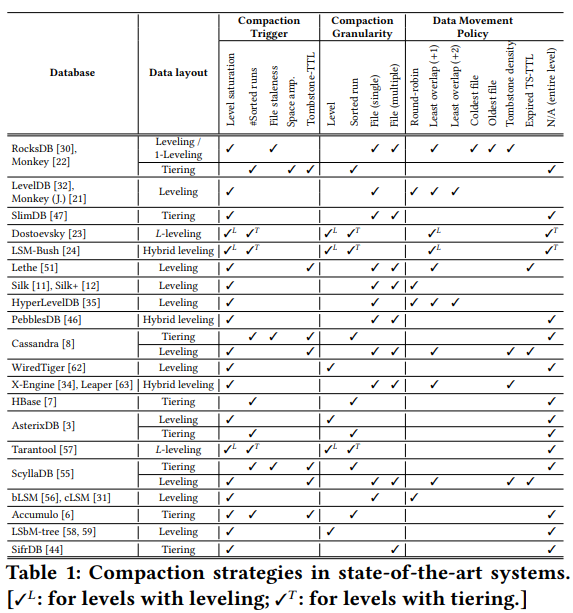
\includegraphics[width=0.6\textwidth]{img/lsm-compaction/various-compaction-strategy.png}
    \caption{既存システムにおけるコンパクションの分類}
    \label{fig:various-compaction-strategy}
\end{figure}

\begin{figure}
    \centering
    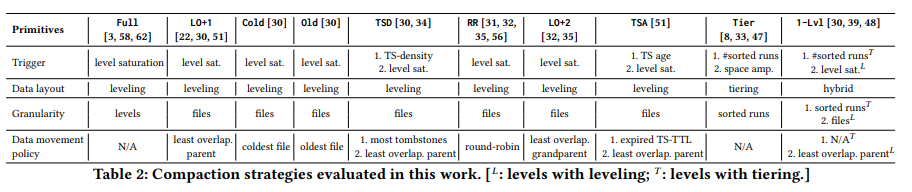
\includegraphics[width=\textwidth]{img/lsm-compaction/target-compaction-strategy.png}
    \caption{今回の論文で評価するコンパクション}
    \label{fig:target-compaction-strategy}
\end{figure}

\section{実験結果}
\begin{experiment}{実験手法}
\begin{itemize}
    \item 実験においてはRocksDBを用いて、様々なコンパクション戦略を実装した。RocksDBはオープンソースであり、学術界でよく利用されている。
    \item 性能評価指標としては以下を用いた。
    \begin{itemize}
        \item コンパクションレイテンシ: 一回のコンパクション処理全体にかかる時間
        \item ライトアンプリフィケーション(WA): データが生存期間中にディスクに書き込まれる回数
        \item ライトレイテンシ: 書き込み処理にかかる時間
        \item リードアンプリフィケーション (RA): 理想的に読むべきページ数に対する、実際にディスクから読みこまれたページ数の比
        \item ポイントルックアップレイテンシ: キーを指定して値を取得する処理にかかる時間
        \item レンジルックアップレイテンシ: 範囲を指定して値を取得する処理にかかる時間
        \item スペースアンプリフィケーション (SA): 論理的に無効化されたエントリのサイズをツリー内のエントリサイズで割った比として定義される。
        \item 削除性能: 指定された時間内に論理削除されたエントリを物理削除できる割合
    \end{itemize}
    \item 評価に用いたワークロードは以下
    \begin{itemize}
        \item データ分布は一様分布、正規分布、Zipf分布
        \item ポイントルックアップでは対象キーがデータベースに存在する場合としない場合、レンジルックアップは選択率で特徴づけられる。上の二つの条件を変えながら評価を行った。
    \end{itemize}
    \item また以下のLSMチューニングパラメータは適切に調節した。それはメモリバッファサイズ、ブロックキャッシュサイズ、ツリーのサイズ比の三つである。
\end{itemize}
\end{experiment}

\begin{experiment}{実験結果}
\begin{itemize}
    \item 結果A.
\end{itemize}
\end{experiment}

\section{感想}
\begin{kansou}
\begin{itemize}
  \item 
\end{itemize}
\end{kansou}

\bibliographystyle{jplain}
\bibliography{template.bib}

\end{document}